\documentclass[11pt,a4paper]{article}
\usepackage[T1]{fontenc}
\usepackage[utf8]{inputenc}
\usepackage{lmodern,amsmath,amssymb,graphicx,booktabs,geometry,hyperref,enumitem}
\geometry{margin=2.3cm}
\hypersetup{colorlinks=true,urlcolor=blue,linkcolor=black,citecolor=black}
\setlength{\parskip}{5pt}\setlength{\parindent}{0pt}
\newcommand{\dd}{\mathrm{d}}
\title{\vspace{-1.5cm}Catatan Turunan\\[2pt]\large Jarak luminositas gelombang gravitasi pada kosmologi Einstein-skalar-Gauss-Bonnet: penurunan dari aksi dan verifikasi}
\author{Afiq Agung\\ {\small Physics, Program Studi Pendidikan Fisika, Universitas Sulawesi Barat, Majene, Indonesia}}
\date{Versi 1.0.0, 21 November 2026}
\begin{document}
\maketitle

\section*{Ringkasan hasil}
\begin{enumerate}[leftmargin=*,itemsep=2pt]
\item Rumus $d_{\rm GW}/d_{\rm EM}=\sqrt{G_T(0)/G_T(z)}$ dengan $G_T=1+8c\,aH$ pada cabang luminal \textbf{terkonfirmasi}: diturunkan dari aksi, diperiksa simbolik dengan dua cara independen, dan diperiksa numerik sampai selisih relatif $10^{-4}$.
\item Tanda deviasi pada gambar hasil awal benar untuk $c>0$: $d_{\rm GW}>d_{\rm EM}$ pada $z\lesssim 2$.
\item Temuan utama: persamaan Friedmann pada cabang luminal adalah $3H^2(1+8c\,aH)=\rho$. Karena $aH$ membesar ke masa lalu, cabang luminal yang berlaku sejak rekombinasi atau nukleosintesis memaksa sinyal di $z<2$ menjadi sangat kecil (Tabel~\ref{tab:plafon}). Sinyal berorde persen hanya mungkin bila kopling baru aktif pada alam semesta akhir.
\end{enumerate}

\section{Konvensi}
Satuan $M_{\rm pl}^2=(8\pi G)^{-1}=1$ dan $c=1$. Aksi
\begin{equation}
S=\int \dd^4x\,\sqrt{-g}\left[\frac{R}{2}-\frac12(\partial\phi)^2-V(\phi)+f(\phi)\,\mathcal{G}\right]+S_{\rm m},\qquad
\mathcal{G}=R^2-4R_{\mu\nu}R^{\mu\nu}+R_{\mu\nu\rho\sigma}R^{\mu\nu\rho\sigma}.
\end{equation}
Fungsi $f$ di sini sama dengan $\xi$ pada naskah lain. Literatur yang menulis $-\tfrac18\xi\,\mathcal{G}$ diperoleh dengan substitusi $f=-\xi/8$. Titik menyatakan turunan terhadap waktu kosmik, $H=\dot a/a$.

\section{Aksi kuadratik tensor}
Metrik uji untuk satu polarisasi yang merambat sepanjang $z$:
\begin{equation}
\dd s^2=-\dd t^2+a^2(t)\left[e^{h}\dd x^2+e^{-h}\dd y^2+\dd z^2\right],\qquad h=h(t,z).
\end{equation}
Karena $\det g_{ij}=a^6$ secara eksak, suku skalar minimal dan materi tidak menyumbang pada orde $h^2$. Ekspansi $\sqrt{-g}\,[R/2+f\mathcal{G}]$ sampai orde kedua memberi persamaan gerak
\begin{equation}
\frac{\dd}{\dd t}\!\left(a^3G_T\,\dot h\right)-a\,F_T\,\partial_z^2h=0,\qquad
G_T=1+8H\dot f,\qquad F_T=1+8\ddot f, \label{eq:tensor}
\end{equation}
tanpa suku massa. Kecepatan tensor adalah $c_T^2=F_T/G_T$.

\textbf{Verifikasi.} (i) Skrip \texttt{check\_tensor\_action.py} menghitung tensor Riemann metrik di atas, mengekspansi Lagrangian, dan mengambil persamaan Euler-Lagrange; koefisien $\ddot h$, $\dot h$, $\partial_z^2h$ cocok dengan \eqref{eq:tensor} dan sisanya nol. (ii) Skrip \texttt{check\_background\_and\_horndeski\_map.py} memperoleh $G_T$ dan $F_T$ yang sama dari peta Horndeski $G_4=\tfrac12+4f''X(2-\ln X)$, $G_5=-4f'\ln X$.

\section{Cabang luminal}
Syarat $c_T=1$ setara dengan $\ddot f=H\dot f$, sehingga
\begin{equation}
\dot f=c\,a,\qquad G_T=F_T=1+8c\,aH=1+\beta\,\frac{aH}{H_0},\qquad \beta\equiv 8cH_0 .
\end{equation}
Syarat ini tidak memerlukan persamaan medan skalar. $G_T>0$ diperlukan agar tensor bebas hantu. Fier dkk. melaporkan bahwa stabilitas menuntut $c\ge 0$; syarat sektor skalar ini \emph{belum} saya turunkan ulang.

\section{Jarak luminositas gelombang gravitasi}
Dalam waktu konformal $\eta$, persamaan \eqref{eq:tensor} pada cabang luminal menjadi $(a^2G_Th')'+a^2G_Tk^2h=0$. Dengan $\chi=a\sqrt{G_T}\,h$ diperoleh $\chi''+\left[k^2-(a\sqrt{G_T})''/(a\sqrt{G_T})\right]\chi=0$, sehingga untuk $k\gg aH$ amplitudo $\chi$ tetap dan $|h|\propto 1/(a\sqrt{G_T})$. Dibandingkan relativitas umum ($|h|\propto1/a$),
\begin{equation}
\boxed{\;\frac{d_{\rm GW}}{d_{\rm EM}}(z)=\sqrt{\frac{G_T(0)}{G_T(z)}}=\left[\frac{1+\beta}{1+\beta\,a(z)H(z)/H_0}\right]^{1/2}\;}
\end{equation}
Ini identik dengan Pers.~(12) Linder (2021). Linder menyimpulkan bahwa Gauss-Bonnet terkopel dengan $c_T=1$ tidak memberi kosmologi inflasi maupun kosmologi akhir zaman yang sah; skenario jendela akhir zaman pada Tabel~\ref{tab:plafon} hanya lolos karena melepas $c_T=1$ di masa lalu. Asumsi yang dipakai: amplitudo di sumber dinormalkan seperti pada relativitas umum, dan pengaruh $G$ efektif lokal pada massa chirp diabaikan.

\textbf{Verifikasi numerik.} Skrip \texttt{check\_distance\_ratio\_numerical.py} mengintegrasikan persamaan gelombang ($k=400H_0$, latar $\Lambda$CDM, $\Omega_m=0{,}3$) untuk $\beta=0{,}1;\,0{,}3;\,0{,}6$ dan $z=0{,}3$ sampai $3$. Selisih relatif terhadap rumus analitik paling besar $1{,}3\times10^{-4}$, sesuai orde koreksi WKB.

\begin{center}
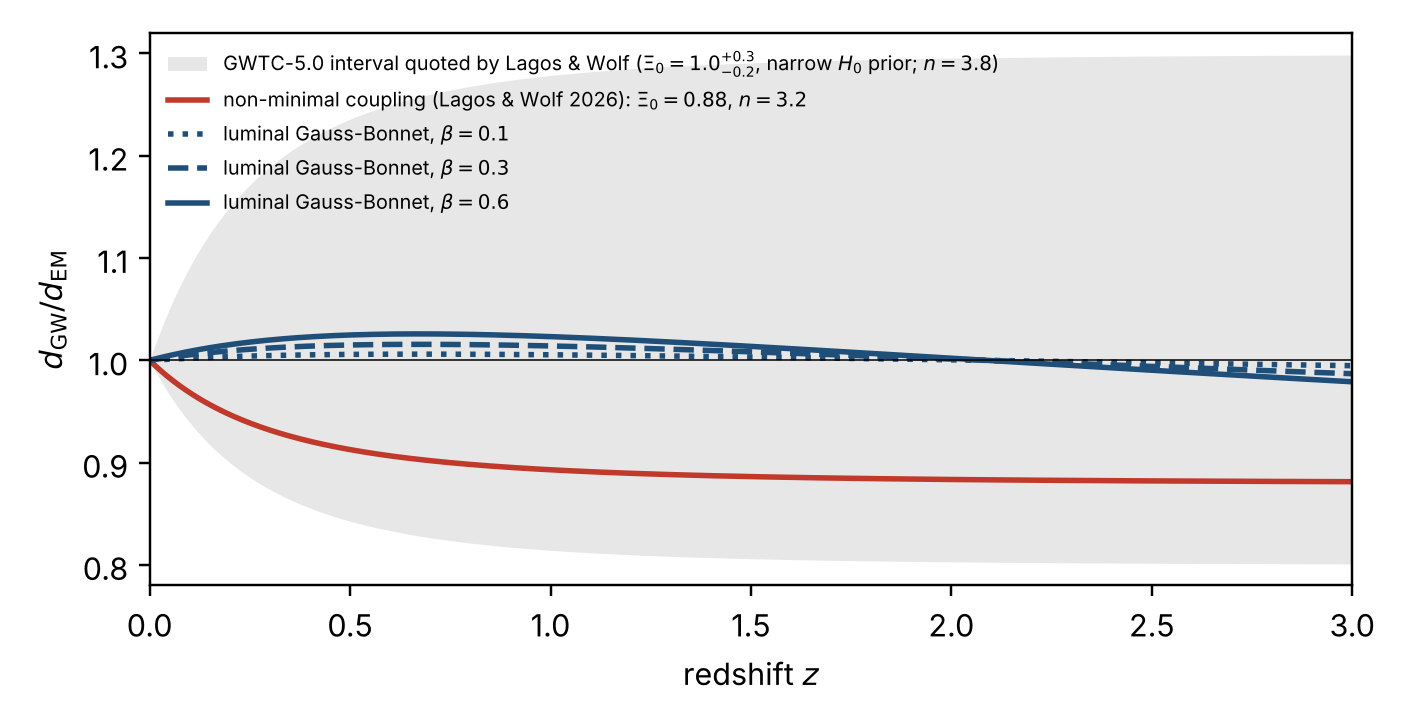
\includegraphics[width=0.8\textwidth]{../figures/ratio_gb_vs_nmc.png}
\end{center}

\section{Persamaan Friedmann pada cabang luminal}
Dengan lapse $N$, $\sqrt{-g}\,\mathcal{G}=\frac{\dd}{\dd t}\!\left(8\dot a^3/N^3\right)$ (terverifikasi simbolik). Variasi terhadap $N$ memberi
\begin{equation}
3H^2\left(1+8H\dot f\right)=\rho_\phi+\rho_{\rm m}\quad\Longrightarrow\quad 3H^2\,G_T=\rho_{\rm tot},\qquad \rho_{\rm tot}=\rho_{\rm m}+\tfrac12\dot\phi^2+V .
\end{equation}
Jadi pada latar, konstanta gravitasi kosmologis efektif adalah $G/G_T$, dan pada cabang luminal $3H^2(1+\beta aH/H_0)=\rho_{\rm tot}$.

\section{Perkiraan awal plafon sinyal}
Bila cabang luminal berlaku sampai suatu zaman dengan toleransi $|G_T-1|\le\epsilon$ di zaman itu, maka $0\le\beta\le\epsilon/(aH/H_0)$ (batas bawah dari syarat stabilitas Fier dkk.; $\epsilon=0{,}05$ di nukleosintesis setara kira-kira $|\Delta N_{\rm eff}|\approx0{,}3$), dan deviasi maksimum di $z<2$ kira-kira $0{,}066\,\beta$ (dari $aH/H_0\simeq0{,}87$ di $z\simeq0{,}67$).

\begin{table}[h]\centering
\caption{Perkiraan orde besaran, bukan hasil akhir. Nilai $\epsilon$ adalah asumsi kerja yang harus diganti dengan batas dari literatur.}\label{tab:plafon}
\small\begin{tabular}{p{4.4cm}cccp{3.6cm}}\toprule
Cabang luminal berlaku sejak & $aH/H_0$ & $\epsilon$ (asumsi) & $\beta$ maksimum & deviasi maksimum, $z<2$\\\midrule
Nukleosintesis ($z\sim4\times10^9$) & $4\times10^{7}$ & 0,05 & $1\times10^{-9}$ & $9\times10^{-11}$\\
Rekombinasi ($z\simeq1100$) & 21 & 0,05 & $2\times10^{-3}$ & $2\times10^{-4}$\\
Hanya alam semesta akhir ($z\lesssim3$) & sekitar 1 & tidak mengikat & ditentukan data & 0,6 sampai 2,6 persen ($\beta=0{,}1$ sampai $0{,}6$)\\\bottomrule
\end{tabular}
\end{table}

\section{Batasan}
\begin{itemize}[leftmargin=*,itemsep=2pt]
\item Anomali berorde persen hanya berlaku untuk kopling yang aktif pada alam semesta akhir. Skenario itu berarti $c_T\neq1$ pada zaman yang lebih awal, dan akibatnya tidak dihitung di sini.
\item Nilai pada Tabel~\ref{tab:plafon} adalah perkiraan orde besaran dengan toleransi $\epsilon$ yang diasumsikan, bukan batas dari analisis data.
\item Batas lokal dari biner kompak (Fier dkk.) jauh lebih kuat daripada perkiraan kosmologis di sini; keduanya bertumpu pada asumsi yang berbeda.
\end{itemize}

\section{Uji templat}
Rasio sektor Gauss-Bonnet dicocokkan ke templat $(\Xi_0,n)$, $d_{\rm GW}/d_{\rm EM}=\Xi_0+(1-\Xi_0)/(1+z)^n$, dan ke templat $c_M$, $\alpha_M=c_M/E^2(z)$, yang memberi $d_{\rm GW}/d_{\rm EM}=\exp\{[c_M/(2\Omega_{\Lambda0})]\ln[(1+z)/(\Omega_m(1+z)^3+\Omega_{\Lambda0})^{1/3}]\}$. Skrip: \texttt{fit\_standard\_templates.py} (latar $\Lambda$CDM, $\beta=0{,}1$ sampai $0{,}6$).

\begin{center}\small
\begin{tabular}{lccc}\toprule
Rentang & sisa maks. $(\Xi_0,n)$ & sisa maks. $c_M$ & dibanding anomali\\\midrule
$z<1$ & 0,07 sampai 0,29 persen & 0,17 sampai 0,72 persen & sekitar sepersepuluh\\
$z<2$ & 0,37 sampai 1,58 persen & 0,43 sampai 1,80 persen & lebih dari separuh\\
$z<3$ & 0,71 sampai 2,92 persen & 0,68 sampai 2,78 persen & setara\\\bottomrule
\end{tabular}
\end{center}
Kesimpulan: pada $z<1$ templat menangkapnya dengan baik ($\Xi_0=1{,}006$ sampai $1{,}027$, $n\simeq5$); kegagalan baru muncul di $z>1$ dan tetap berorde persen. Rumus templat $c_M$ dicocokkan dengan Pers.~(7) sampai (9) Lagos dan Wolf; dengan $c_M=-0{,}5$ rumus ini memberi rasio asimtotik 0,87, sesuai nilai 0,88 mereka. Sirene tidak dapat memisahkan Gauss-Bonnet luminal dari relativitas umum; yang terpisahkan adalah kopling non-minimal dari keduanya.

\section{Status verifikasi}
\begin{tabular}{p{9.2cm}p{5.6cm}}\toprule
Pernyataan & Status\\\midrule
$G_T=1+8H\dot f$, $F_T=1+8\ddot f$ & simbolik, dua cara\\
$c_T=1\Leftrightarrow\dot f=ca$ & simbolik\\
$d_{\rm GW}/d_{\rm EM}=\sqrt{G_T(0)/G_T(z)}$ & analitik (WKB) dan numerik\\
$3H^2G_T=\rho_{\rm tot}$ & simbolik (minisuperspace)\\
Syarat $c\ge0$ dari sektor skalar & belum, dikutip dari Fier dkk.\\
Nilai $\epsilon$ pada Tabel 1 & belum, perlu rujukan\\
Latar pada gambar ($\Lambda$CDM) & pendekatan; latar EsGB swakonsisten belum dipakai\\\bottomrule
\end{tabular}

\section*{Rujukan yang dipakai}\raggedright
Linder EV, arXiv:2108.11526 (2021). Fier J dkk., arXiv:2503.01975 (2025). Kobayashi T, Yamaguchi M, Yokoyama J, Prog. Theor. Phys. 126 (2011) 511, doi:10.1143/PTP.126.511, arXiv:1105.5723. Lagos M, Wolf WJ, arXiv:2609.04112 (2026).
\end{document}
